\documentclass[a4paper,fleqn]{cas-dc}

%%%Author definitions
\def\tsc#1{\csdef{#1}{\textsc{\lowercase{#1}}\xspace}}
\tsc{WGM}
\tsc{QE}
\tsc{EP}
\tsc{PMS}
\tsc{BEC}
\tsc{DE}
%%%

\usepackage[square,numbers,sort&compress,comma]{natbib}

\usepackage{amsmath}
\usepackage{amssymb}
\usepackage{diagbox}
\usepackage{caption}
\usepackage{graphicx}
\usepackage{latexsym}
\usepackage{times}
\usepackage[pagewise]{lineno}
\graphicspath{{figures/}}
\usepackage{color, colortbl}
\usepackage{chemformula}
\usepackage{xcolor}
\definecolor{Gray}{gray}{0.9}
\newcommand{\highlight}[1]{%
  \colorbox{Gray}{$\displaystyle#1$}}
\usepackage{color, colortbl}
\usepackage{chemformula}
\usepackage{xcolor}
\usepackage{adjustbox}
\usepackage{mathrsfs}
\usepackage{booktabs}
\usepackage{hyperref}
\usepackage{lipsum}

\emergencystretch = 0 pt
\pretolerance = 150
\tolerance = 250
\hbadness = 150
\hfuzz = 0 pt
\vfuzz = 0 pt

\newcommand{ \kamila}[1]{\color{blue}{Kamila: #1} \color{black}}
\newcommand{ \todump}[1]{\color{olive}{#1} \color{black}}
\usepackage[normalem]{ulem}

\begin{document}

\shorttitle{\texttt{pykitPIV}: PyTorch-compatible synthetic image generation for particle image velocimetry}
\shortauthors{Zdyba\l{} et~al.}


\title [mode = title]{\texttt{pykitPIV}: PyTorch-compatible synthetic image generation for particle image velocimetry}

\author[EMPA]{Kamila Zdyba\l{}*}
\ead{kamila.zdybal@gmail.com}

\author[EMPA]{Claudio Mucignat}
\author[EMPA]{Ivan Lunati}

\address[EMPA]{Laboratory for Computational Engineering, Swiss Federal Laboratories for Materials Science and Technology, Empa, Dübendorf, Switzerland}


\begin{abstract} 
We describe pykitPIV
\end{abstract}

\begin{keywords}
progress variable; ammonia; parameterization; flamelet-like model; low-dimensional manifold; artificial neural network
\end{keywords}

\maketitle

\section{Introduction\label{sec:introduction}}



\begin{figure}[t]
\centering
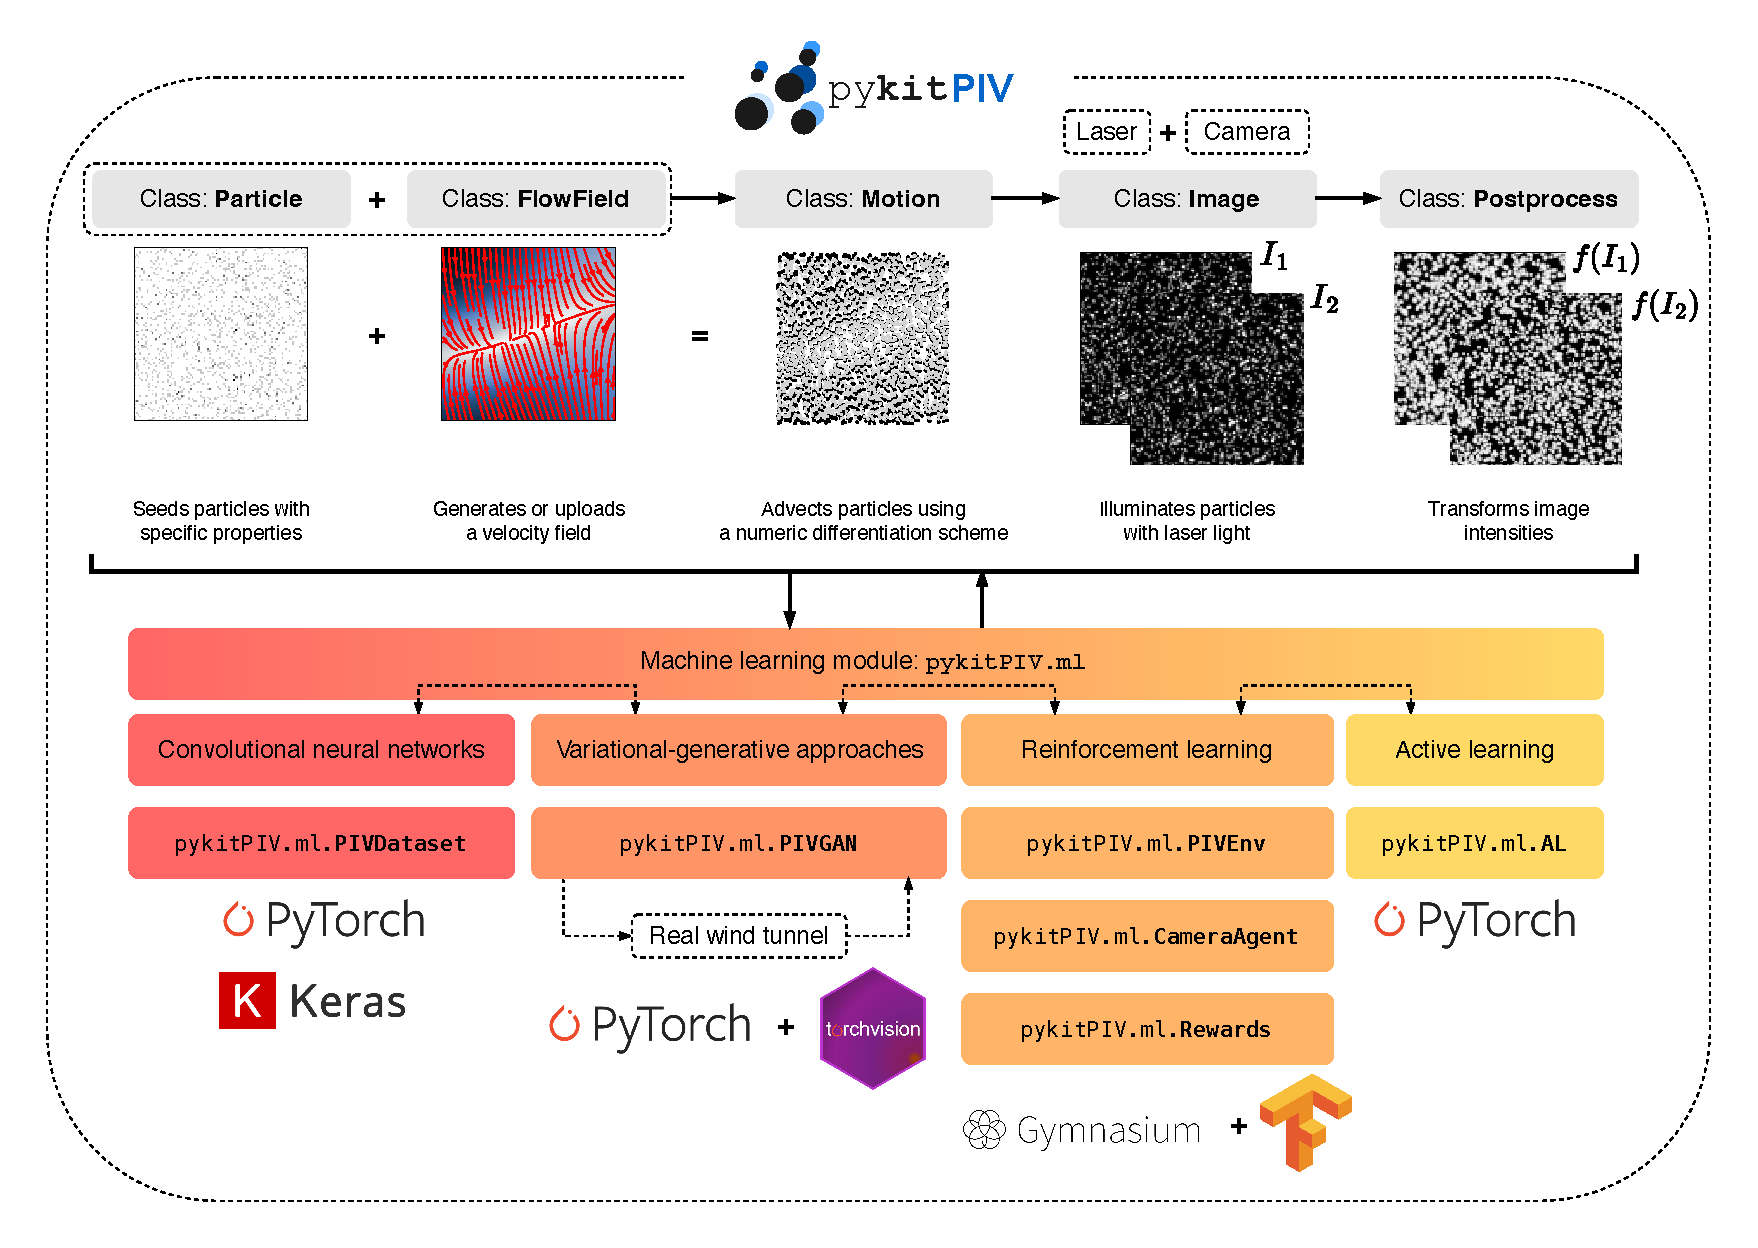
\includegraphics[width=7cm]{pykitPIV-modules.pdf}
\caption{Order of using pykitPIV modules.}
\label{fig:pykitPIV-modules}
\end{figure}




\section{Results and discussion} \label{sec:results}


\begin{figure*}[t]
\centering
\vspace{-0.4 in}
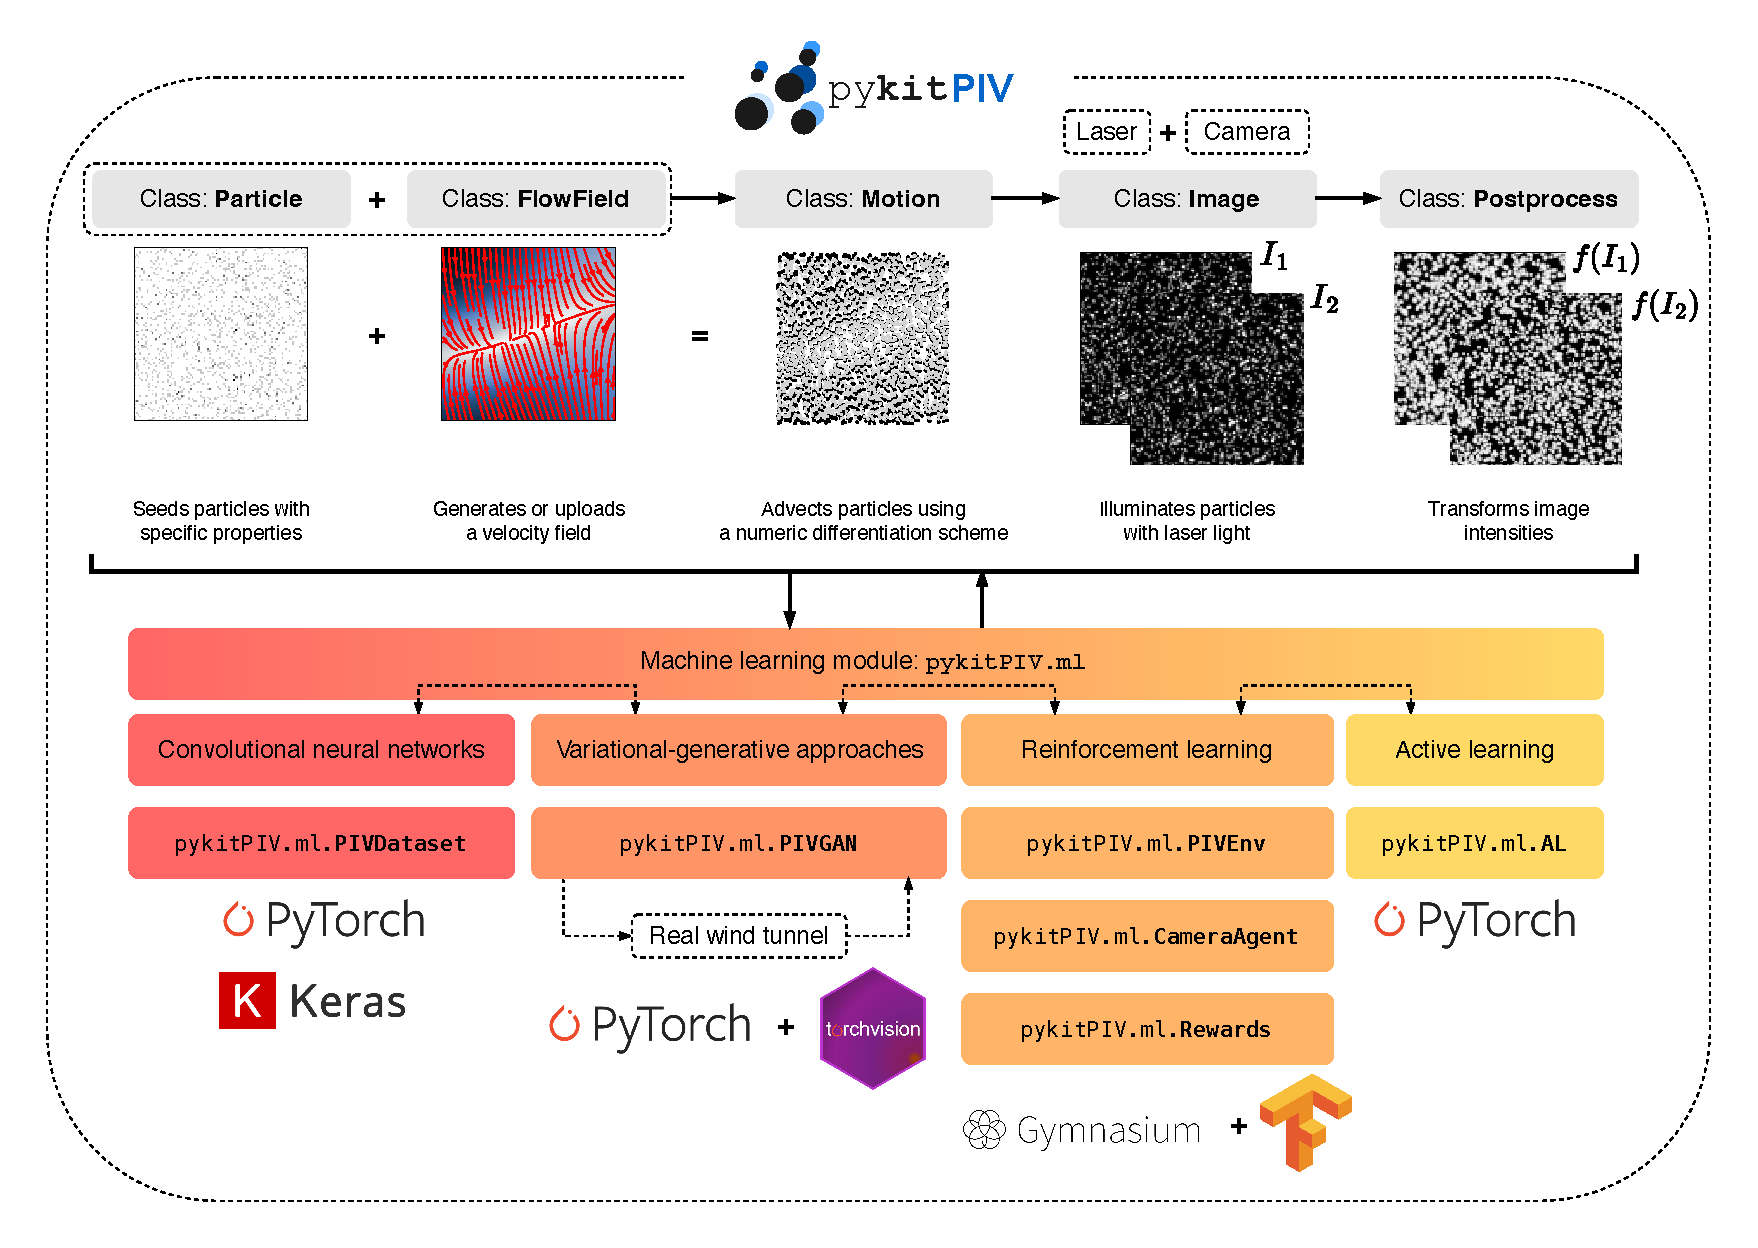
\includegraphics[width=\textwidth]{pykitPIV-modules.pdf}
\vspace{10 pt}
\caption{\footnotesize The variety of operations on PIV images possible with the pykitPIV modules.}
\label{fig:operations}
\end{figure*}


\section{Conclusions}



\section*{Declaration of competing interest}

The authors declare that they have no known competing financial interests or personal relationships that could have appeared to influence the work reported in this paper.

\section*{Author contributions}



\section*{Acknowledgments}




\bibliographystyle{pci}
\bibliography{bibliography}

\end{document}